\cotefile{150}

\scanpage{79}
\mspage{35}
Si $J$ est un ``idéal'' i.e. $\unsure{i|\deleted{x}\inserted{i}}\in J$, $j<i\Longrightarrow j\in J$,
alors on a $X_J^*=X_J$, donc $X_J^*$ est fermé.

Si $J$ est une ``bande'' i.e. si $i,j\in J$, $i<j$,
alors $\forall k\in I$, $(i<k<j\Longrightarrow k\in J)$,
ou ce qui revient au $=$, si $J'=\widetilde J\setminus J$ est
un ``idéal'', où $\widetilde J$ est l'idéal engendré par $J$,
alors on a
\[
(59)\qquad X_J^*=X_{\widetilde J}^*\setminus X_{J'}^*
\]
\deleted{$=X_{\unsure{\widetilde J|J}}^*$}.
\margin{différence de deux parties fermées, c'est une partie
loc\textsuperscript{t} fermée de $X$}
dont les $X_i^J\overset{\mathrm{déf}}{=}X_i\cap X_J^*$ ($i\in J$)
forment une stratification. Posons
\[
(60)\qquad V_{j_0-j_n}^J
=V_{j_0\mathord{-}\mathord{-}j_n}\cap X_J^*=V_{j_0-j_n}^Z
\qquad\text{pour }Z=X_J^*
\]
pour $j_0\unsure{\ast|\ne}\mathord{-}j_n\in J$, $j_0<j_1<\mathord{-}\mathord{-}<j_n$,
\deleted{dans la}
ce sont alors les $V_{i_0\mathord{-}\mathord{-}i_n}$ associés à la stratification
de type $J$ de $X_J^*=Z$. On a donc
\[
(61)\qquad\begin{aligned}
X_J^*&\simeq\underset{i,j\in J}{\unsure{\uline{\lim}|\varinjlim}}
(V_i^J,V_{ij}^J)\\
&\simeq\underset{\substack{(i_0\unsure{<|\leq}\mathord{\cdot}\mathord{-}\unsure{<|\leq}i_n)\\\in\operatorname{Drap}(J)}}{\unsure{\uline{\lim}|\varinjlim}}
(V_{i_0\mathord{-}\mathord{-}i_n}^J)
\end{aligned}
\]
\deleted{On s'intéresse à la situation de}
\margin{78}

\scanpage{81}
\mspage{36}

\deleted{Le cas ou $V$}

Posons, pour une bande $J$
\[
\begin{aligned}
(62)\qquad V_J&=\text{provoisinage tubulaire de }X_J^*\text{ dans }X\\
&=\bigcup_{i\in J}V_i=\varinjlim_{i,j\in J}(V_i,V_{ij})
\end{aligned}
\]
On s'intéresse aux protopos de la forme
\[
(63)\qquad V_J^L\overset{\mathrm{def}}{=}V_J\cap X_L^*,
\]
\margin{\uline{Ex} $J\subset\deleted{J'}\inserted{K\ \text{(idéal de $J'$)}}$ inclusion de bandes, \deleted{\unsure{disposition}} $X_J^*\subset X_{J'}^*$, on prend
$V(X_J^*,X_{J'}^*)\setminus V(X_J^*,X_{J'}^*)\cap X_K^*$}
\margin{protopos de raccord entre $X_J^*$ et $X_L^*$
\diagram{\begin{tikzcd}[column sep=small,row sep=small]
V_J^L\arrow[r,hook]\arrow[d,hook]&X_L^*\arrow[r,hook]&V_L\\
V_J&&
\end{tikzcd}}
\deleted{\unsure{NB} $V_J^{\unsure{L}}\cap V_{J'}^{L'}=V_{J\cap J'}^{L\cap L'}$}}
où $J,L$ sont deux bandes. Par exemple on retrouve les $X_J^*$ comme
\[
(64)\qquad V_J^J=X_J^*
\]
Soit $L_0\subset L$ \unsure{l'ens|) l'ens} des $l\in L$ qui majorent un \unsure{élém|élément} de $J$, et $J_0$ l'ens des $j\in J$ qui mino-\\rent un élément de $L$, on a donc
\[
(65)\qquad V_J^L=V_J^{L_0}=V_{J_0}^L=V_{J_0}^{L_0}
\]
où $J_0,L_0$ sont des sous-bandes de $J,L$ respectivement ($J_0$ est = un idéal de $J$, $L_0$ un coidéal de $L$) telles que tt élément de $J_0$ est majoré par un élément de $L_0$, tt élément de $L_0$ majore un élément de $J_0$. On est ainsi ramené au cas de bandes dans la relation de domination
\[
(66)\qquad J\prec L
\]
\margin{qui signifie que tt élément de $J$ majoré par un élément de $L$, tt \unsure{élément|élémt} de $L$ majore un él. de $J$.}
\unsure{de|donc}
% The light, thin bottom-left foliation is in another hand.
\margin{80}

\scanpage{82}
\mspage{37}

\uline{Lemme} Soient $I$ un ens ordonné, $J,L$ deux parties de $I$. Conditions équivalentes

a) $1^{\mathrm o})$ $J,L$ sont des bandes, $2^{\mathrm o})$ tout élément de $J$ est majoré par un élément de $L$, tout élément de $L$ majore un élément de $J$, \deleted{$3^{\mathrm o})$ si $j\in J$, $l\in I$ sont tels que $l\leq j$, alors $j,l\in J\cap L$}
\margin{ie $J\prec L$}

b) $\exists$ une bande $I'$ de $I$, telle que $J$ soit un idéal de $\unsure{{}'I'|I'}$, $L$ un coidéal de $I'$, et que tout élément de $I'$ majore un élément de $J$ et soit majoré par un élément de $L$.

Sous ces conditions, \deleted{il existe \unsure{une} plus} \inserted{la bande $I'$ de b) est unique,} \unsure{et|c'est} la plus petite petite bande \inserted{$I'$} contenant $J$ et $L$ satisfait b), et est donnée par
\[
(67)\qquad I'=\{i\in I\mid\exists j\in J,l\in L\text{ avec }j\leq i\leq l\}
\]

\uline{Dém} L'implication b) $\Rightarrow$ a) triviale, \inserted{ainsi que le fait que $I'$ est \unsure{donné|donnée} par (\unsure{67})} prouvons a) $\Rightarrow$ b). Soit $I'$ donné par (67), on a $I'\supset J\cup L$ (par a) $2^{\mathrm o})$) $I'$ est une bande (trivial), et c'est évidemment la plus petite bande $\supset J\cup L$. Prouvons que $J$ est un idéal de $I'$ i.e. $j\in J$, $i\in I'$, $i\leq j\Rightarrow i\in J$\unsure{..|.} Comme $i\in I'$, $\exists j_0\in J$ tel que $j_0\leq i$, donc $j_0\leq i\leq j$ avec $j_0,j\in J$, et comme $J$ est une bande \inserted{(par a $1^{\mathrm o}$)} on a $i\in J$. On voit directement que $I$ est un coidéal de $I'$. Soit $i\in I'$, \deleted{de \unsure{par}} \inserted{par} définition de $I'$ $i$ majore un élément de $I$ et est majoré par un élément de $L$, qfd.
\margin{\handwritten{81}}

\scanpage{83}

Dans le cas actuel, on aura donc
\[
\begin{aligned}
(68)\qquad V_J^L\simeq{}&\text{le \unsure{proespace|\deleted{t}proespace} de la forme }V_J^{\prime L},\text{ relatif}\\
&\text{à l'espace }X'=X_{I'}^*,\text{ stratifié par les }X_i'\\
&X_i'\doteq X_i\cap X_{I'}^*\quad(i\in I'),\text{ où }X_J'\text{ est fermé,}\\
&\text{et }X_L'\text{ est ouvert, }\deleted{\text{et }\unsure{\text{où}|\text{aussi}|\text{ainsi}}}
\end{aligned}
\]
(Car on a
\[
V_J^L=V_J\cap X_L^*
=\left(\bigcup_{j\in J}V_j^{X'}\right)\cap
\left(\overbrace{\bigcup_{l\in L}V_{\deleted{j}\inserted{l}}^{X'}}^{\substack{\inserted{X_L^*\ \text{car }X_L^*\text{ ouvert dans }X'}\\\Vert}}\right)
=\bigcup_{j\in J,l\in L}V_{j,l}^{X'}
\]
Notons que
\[
\begin{aligned}
V_{j,l}^{X'}&=
\begin{cases}
\varnothing&\text{si }j,l\text{ non comparables}^*\\
V_j^{X'}&\text{si }j=l,\text{ et donc }j,l\in J\cap L\\
V_{j,l}^{X'}\ \text{standard}&\text{si }j<l\\
V_{l,j}^{X'}\ \text{standard}&\text{si }l<j\text{ donc }l,j\in J\cap L
\end{cases}\\
&\qquad\qquad\text{(donc }l\in J,j\in L\text{ !)}
\end{aligned}
\]
\margin{$^*$ sous réserve que les ouverts de $X$ soient normaux, p.ex. $X$ métrisable....}
donc
\[
(69)\qquad V_J^L=\bigcup_{\substack{j\in J\\l\in L\\j\leq l}}V_{j,l}^{X'}\qquad\deleted{\text{\unsure{pour}}}
\]
(où on se rappellera que $V_{j,j}^{X'}=V_j^{X'}$)

\margin{\uline{NB} Sur cette formule, valable si $J\prec L$, on voit que dans ce cas on a (équiv. d'homotopie)
\diagram{\begin{tikzcd}[column sep=large,row sep=small]
V_J^L\arrow[r,"{\substack{(h)\\[-.4ex]\sim}}"]\arrow[d,equal,"{\mathrm{déf}}"']&\underbrace{V_J\cap V_L}_{\underset{(\mathrm{déf})}{=}V_{J,L}}\\
V_J\cap X_L^*&
\end{tikzcd}}}

Pour écrire $V_J^L$ par \uline{recollement} des $V_{j,l}^{X'}$, il faut expliciter les
\[
V_{j,l}^{X'}\cap V_{j',l'}^{X'}
\]
qui sont vides, sauf si $\{j,j',l,l'\}$ est un drapeau. C'est un drapeau \deleted{\unsure{de|dont|donc}} ayant au plus quatre termes \inserted{(distincts)}, \deleted{qui} \inserted{ceux-ci} sont dans $J\cup L$, et il en est au \deleted{moins deux dans $J$, deux dans $L$, et au moins un} moins un dans $J$, au moins un dans $L$. Ce sont donc des drapeaux de la forme
\margin{82}

\scanpage{84}
\mspage{38}

\[
(70)\quad\left\{\begin{array}{lll}
V_i^{X'}&i\in J\cap L&\\
V_{ij}^{X'}&i\in J\inserted{\setminus J\cap L},\ j\in L\setminus J\cap L&(i<j)\\
V_{ijk}^{X'}&i\in J,\ k\in L,\ j\in J\cup L&(i<j<k)\\
V_{ijkl}^{X'}&i,j\in J,\ k,l\in L&(i<j<k<l)
\end{array}\right.
\]

\margin{\uline{NB} le cas le plus intéressant est celui où $J\cap L=\phi$ Et ça se \unsure{réduit} donc par \unsure{cas} dans (70)\unsure{,} où le cas $V_i^{X'}$ --- \unsure{inutile et peu} \inserted{il reste \unsure{moins conclusif}} \uline{quatre} \uline{cas}}

On peut donc dire que $V_J^L$ est la $\varinjlim$ (finie) des proespaces précédents, avec \deleted{les} les morphismes semi-simpliciaux \deleted{qui en \unsure{résultent|explicite}} \inserted{entre ces espaces}.

\deleted{On a \unsure{les} $\unsure{V_{ijk}}$}
Si on veut un système \deleted{semi-simplicial} des proespaces, \inserted{stable par intersections} qui par \deleted{\unsure{recollement}} \inserted{$\unsure{\varinjlim|\underline{\lim}}$} donne $V_J^L$, on prendra les

\[
(71)\qquad V_{i_0\mathord{\cdot}\mathord{-}i_n}^{X'}\quad\text{avec }i_0<\mathord{\cdot}\mathord{-}<i_n,\qquad
\left\{\begin{array}{l}
i_0,\mathord{\cdot}\mathord{\cdot}i_n\in J\cup L\\
i_0\in J,\ i_n\in L
\end{array}\right.
\]

\deleted{\unsure{au lieu de}}
les flèches entre ces espaces correspondent aux inclusions de drapeaux \uline{satisfaisant} les \uline{conditions précédentes}. Posons donc

\[
(72)\qquad\operatorname{Drap}_J^L(I)\subset\operatorname{Drap}(\unsure{J\deleted{\}}}\cup L)\subset\operatorname{Drap}(I)
\]

drapeaux \inserted{``$(i_0-i_n)$} qui sont tels que $i_0\in J,i_n\in L$

On a donc un recouvrement de $V_J^L$ par les $V_d^{X'}$, où $d$ parcourt l'ens ordonné précédent. On aura p.ex, pour un faisceau $F$ sur $V_J^L$

\[
(73)\qquad H^*(V_J^L,F)\Longleftarrow E_2^{pq}=H^p(\operatorname{Drap}_J^L(I),d\to H^q(V_d^{X'},F)\unsure{)}
\]

\margin{83}

\scanpage{85}

\noindent\uline{16}\quad $\Sigma_J$ et $\Sigma_{J,L}$.

\margin{Un point de vue peut-être plus commode pour définir les $\Sigma_i$, $\Sigma_{i_0\ldots i_n}$, $\Sigma_J$, $\Sigma_J^{L}$ est celui des ``éclatés orientés'', mieux adapté à des formules du type $X=\underset{d\in\mathrm{Drap}(I)}{\uline{\lim}}\Sigma_d$. On prend des $\Sigma_i\supset X_i^*$ et non $\deleted{\unsure{\Sigma_i}}\subset X_i^*$, \unsure{idem pour} $\Sigma_J$, $X_J^*=\Sigma_J\setminus\dot\Sigma_J$\ldots}

Soit $J$ une bande de $I$, on définit
\[
(70)\qquad
\begin{array}{@{}l@{}}
\Sigma_J\subset X_J^*\\[-.4ex]
\hspace{.6em}\Vert\\[-.4ex]
X_J^*\setminus X_J^*\cap\displaystyle\bigcup_{i\in\bar J\setminus J}\mathring T_i
\end{array}
\]
\[
\begin{array}{@{}c@{\quad}l@{}}
\deleted{\Vert}&\Vert\quad\text{\uline{NB}}\\[-.4ex]
\deleted{\displaystyle\bigcup_{j\in J}\Sigma_j}&
X_J^{\deleted{\unsure{*}}}\setminus X_J^{\deleted{\unsure{*}}}\cap\displaystyle\bigcup_{i\in\bar J\setminus J}T_i
\end{array}
\]
\margin{NB $\bar J=$ idéal engendré par $J$ $=\{i\in I\mid\exists j\in J\ \text{avec}\ i\leq j\}$}
\margin{\uline{NB} On a posé $X_J=\bigcup_{j\in J}X_j\ (=\bigcup_{j\in\bar J}X_j^*=X_{\bar J}^*)$}

On a donc
\[
(71)\quad\left\{
\begin{aligned}
\Sigma_{\phi}&=\phi,\quad\Sigma_{\{j\}}=\Sigma_j,\quad\Sigma_I=X\\
\Sigma_J&=X_J\quad\text{si $J$ un idéal i.e. $J=\bar J$}
\end{aligned}\right.
\]

On a même, sauf erreur
\[
(72)\qquad\Sigma_J\simeq\underset{i,j\in J}{\lim_{\longrightarrow}}\left(\Sigma_j,\Sigma_{ij},\deleted{\unsure{b}}(s_{ij},b_{ij}:\right.
\]
\diagram{\begin{tikzcd}[ampersand replacement=\&,column sep=small,row sep=small]
\&\Sigma_i\\
\Sigma_{ij}\arrow[ur]\arrow[dr]\&\\
\&\Sigma_j
\end{tikzcd}}
\[
\left.\vphantom{\Sigma_{ij}}\right)\qquad\simeq\underset{d\in\mathrm{Drap}(J)}{\uline{\lim}}\Sigma_d
\]
\margin{\uline{NB} $\Sigma_J$ est muni d'une stratification de type $J$, que \unsure{l'on déduit} des $(\Sigma_j,\Sigma_{jh},s_{jh},b_{jh})$ avec $j,h\in I$}
\deleted{Par suite \unsure{d'un}}
\[
(73)\qquad\Sigma_J\overset{\overset{h}{\sim}}{\hookrightarrow}X_J^*\qquad(\text{équivalence d'homotopie})
\]

On pose
\[
(74)\qquad\begin{aligned}
\dot\Sigma_J&=X_J\cap\left(\text{bord de }\underbrace{T_{\bar J\setminus J}}_{\displaystyle\bigcup_{i\in\bar J\setminus J}T_i}\right)\\
&=\bigcup_{\substack{i<j\\i,j\in J}}\operatorname{Im}(\Sigma_{ij}\to\Sigma_J)\\
&=\underset{\substack{d\in\mathrm{Drap},\ d\text{ \unsure{ayant|avec} au moins 2 termes}}}{\lim_{\twoheadrightarrow}}\Sigma_d
\end{aligned}
\]
% Thin lower foliation, in another hand; not the author's page number.
\margin{84}

\scanpage{86}
\mspage{39}

\margin{Je ne suis pas très sûr que l'hypothèse que $J\cap L=\phi$ soit vraiment essentielle, ou celle que $J\prec L$, \unsure{en fait on} dans ces passages.}

Soient $J$ et $L$ deux bandes \uline{disjointes}, avec $J\prec L$ dans une bande $I'$ telles que $J$ est un idéal de $I'$, $L$ un coidéal de $I'$,
\[
I'\subset\widetilde J\cap\bar L\qquad(\text{en fait on aura alors }I'=\widetilde J\cap\bar L)
\]
Soit $J'=I'\setminus L$, donc dans $I'$ on a une inclusion d'idéaux
\[J\subset J'\subset I'\]
(car $J\cap L=\phi$). Considérons \deleted{$X_J^*\subset X_{J'}^*$} le diagramme

\margin{$\Sigma_{JL}=\dot T_J\cap\Sigma_L$, où
\[
\begin{aligned}
T_J&\overset{\mathrm{déf}}{=}\deleted{\unsure{T_J\cap\Sigma_J}}\ ;\ \Sigma_J\cap\bigcup_{j\in J}\unsure{\bar T_j|T_j}\\
\mathring T_J&=\mathring T_{\bar J}\cap\Sigma_J=\Sigma_J\cap\bigcup_{j\in J}\mathring T_j,\\
\dot T_J&=T_J\setminus\mathring T_J,\\
\dot T_J&\overset{?}{=}\underset{\substack{d\in\mathrm{Drap}(I)\\\text{él. initial de }d\text{ est}\in J}}{\lim_{\longrightarrow}}\Sigma_d\quad(=\Sigma_{J,I}),\\
\Sigma_{J,L}&\overset{?}{=}\underset{\substack{\text{él. initial de }d\text{ est}\in J\\\text{--- final \deleted{\unsure{est}}}\in L\\d\in\mathrm{Drap}(J\cup L)}}{\lim_{\longrightarrow}}\Sigma_d
\end{aligned}
\]}

\diagram{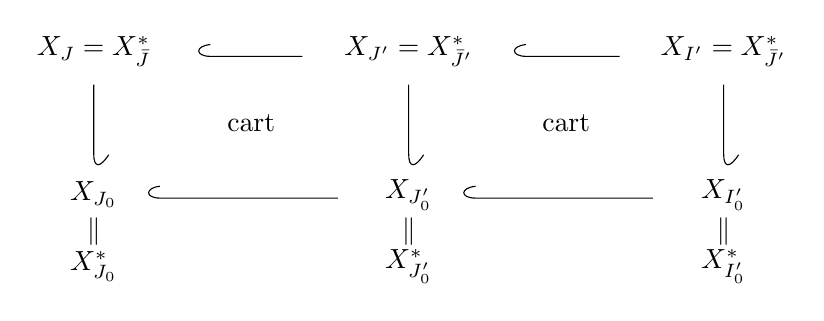
\begin{tikzpicture}[x=1cm,y=1cm]
\node at (0,0) {$X_J=X_{\bar J}^*$};
\node at (4,0) {$X_{J'}=X_{\bar J'}^*$};
\node at (8,0) {$X_{I'}=X_{\bar J'}^*$};
\draw (1.48,0.09) .. controls (1.28,0.07) and (1.29,-0.06) .. (1.48,-0.06) -- (2.65,-0.06);
\draw (5.49,0.09) .. controls (5.29,0.07) and (5.30,-0.06) .. (5.49,-0.06) -- (6.68,-0.06);
\draw (0,-0.42) -- (0,-1.30) .. controls (0,-1.48) and (0.08,-1.48) .. (0.19,-1.31);
\draw (4,-0.42) -- (4,-1.30) .. controls (4,-1.48) and (4.08,-1.48) .. (4.19,-1.31);
\draw (8,-0.42) -- (8,-1.30) .. controls (8,-1.48) and (8.08,-1.48) .. (8.19,-1.31);
\node at (2,-0.90) {cart};
\node at (6,-0.90) {cart};
\node at (0,-1.82) {$X_{J_0}$};
\node at (4,-1.82) {$X_{J'_0}$};
\node at (8,-1.82) {$X_{I'_0}$};
\draw (0.84,-1.71) .. controls (0.65,-1.73) and (0.65,-1.86) .. (0.84,-1.86) -- (3.10,-1.86);
\draw (4.85,-1.71) .. controls (4.65,-1.73) and (4.65,-1.86) .. (4.85,-1.86) -- (7.10,-1.86);
\node at (0,-2.28) {$\Vert$};
\node at (4,-2.28) {$\Vert$};
\node at (8,-2.28) {$\Vert$};
\node at (0,-2.73) {$X_{J_0}^*$};
\node at (4,-2.73) {$X_{J'_0}^*$};
\node at (8,-2.73) {$X_{I'_0}^*$};
\end{tikzpicture}}

correspondant au diagramme
\diagram{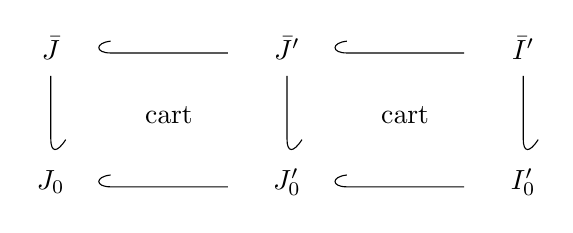
\begin{tikzpicture}[x=1cm,y=1cm]
\node at (0,0) {$\bar J$};
\node at (3,0) {$\bar J'$};
\node at (6,0) {$\bar I'$};
\draw (0.76,0.09) .. controls (0.56,0.07) and (0.56,-0.06) .. (0.76,-0.06) -- (2.25,-0.06);
\draw (3.76,0.09) .. controls (3.56,0.07) and (3.56,-0.06) .. (3.76,-0.06) -- (5.25,-0.06);
\draw (0,-0.35) -- (0,-1.15) .. controls (0,-1.33) and (0.08,-1.33) .. (0.19,-1.16);
\draw (3,-0.35) -- (3,-1.15) .. controls (3,-1.33) and (3.08,-1.33) .. (3.19,-1.16);
\draw (6,-0.35) -- (6,-1.15) .. controls (6,-1.33) and (6.08,-1.33) .. (6.19,-1.16);
\node at (1.5,-0.85) {cart};
\node at (4.5,-0.85) {cart};
\node at (0,-1.70) {$J_0$};
\node at (3,-1.70) {$J'_0$};
\node at (6,-1.70) {$I'_0$};
\draw (0.76,-1.61) .. controls (0.56,-1.63) and (0.56,-1.76) .. (0.76,-1.76) -- (2.25,-1.76);
\draw (3.76,-1.61) .. controls (3.56,-1.63) and (3.56,-1.76) .. (3.76,-1.76) -- (5.25,-1.76);
\end{tikzpicture}}

où
\[J_0=\bar J\setminus J,\qquad J'_0=\bar J'\setminus J',\quad I'_0=\bar I'\setminus I'.\]

On a les inclusions
\diagram{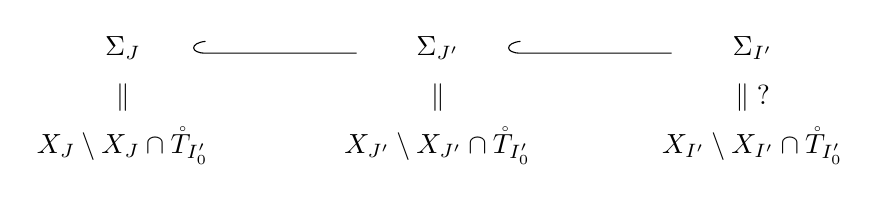
\begin{tikzpicture}[x=1cm,y=1cm]
\node at (0,0) {$\Sigma_J$};
\node at (4,0) {$\Sigma_{J'}$};
\node at (8,0) {$\Sigma_{I'}$};
\draw (1.05,0.09) .. controls (0.85,0.07) and (0.85,-0.06) .. (1.05,-0.06) -- (2.97,-0.06);
\draw (5.05,0.09) .. controls (4.85,0.07) and (4.85,-0.06) .. (5.05,-0.06) -- (6.97,-0.06);
\node at (0,-0.62) {$\Vert$};
\node at (4,-0.62) {$\Vert$};
\node at (8,-0.62) {$\Vert\;?$};
\node at (0,-1.24) {$X_J\setminus X_J\cap\mathring T_{I'_0}$};
\node at (4,-1.24) {$X_{J'}\setminus X_{J'}\cap\mathring T_{I'_0}$};
\node at (8,-1.24) {$X_{I'}\setminus X_{I'}\cap\mathring T_{I'_0}$};
\end{tikzpicture}}
Considérons donc le voisinage tubulaire de $\Sigma_J$ dans $\Sigma_{I'}$
\margin{85}

\scanpage{87}
\mspage{40}

\[
(75)\qquad T_{\Sigma_J,\Sigma_{I'}}=\Sigma_{I'}\cap\bigcup_{j\in J}T_j\left(=\Sigma_{I'}\cap\bigcup_{\deleted{\unsure{j}}j\in\unsure{\bar I|\bar J}}T_j\right)
\]
% The following note is linked by a descending leader to the parenthetical equals sign in (75).
\margin{mais en général c'est différent\ldots}

et considérons son bord
\[
(76)\qquad\dot T_{\Sigma_J,\Sigma_{I'}}=
\underset{\substack{d\in\mathrm{Drap}(I')\\\text{premier terme de }d\text{ est}\in J\\\text{dernier terme est dans }I'\setminus J}}{\lim_{\longrightarrow}}
\left(\Sigma_{\underset{\deleted{\unsure{\uparrow}}}{d}}\right)
\deleted{\underset{\substack{\unsure{\uparrow}\\I'\setminus J}}{\unsure{\cap}}\ \Sigma_{\underset{\substack{\unsure{\uparrow}\\J}}{i_0},i_1,i_2}}
\]
\margin{$(\simeq\Sigma_{J,I'-J}^{\deleted{\unsure{\flat}}}$ avec la notation ci-dessous $(77))$}

On pose (pour $L=I'\setminus J$, rappelons-le)
\[
(77)\quad\left\{
\begin{aligned}
\Sigma_{J,L}^{\unsure{\flat|\natural|\deleted{\flat}|\deleted{\natural}}}&=\dot T_{\Sigma_J,\Sigma_{I'}}\setminus
\underbrace{\dot T_{\Sigma_J,\Sigma_{I'}}\cap
\underbrace{\mathring T_{\overset{\deleted{-}}{J}'}}_{\displaystyle\bigcup_{\deleted{\unsure{\forall}}j\in\overset{\deleted{-}}{J}'}\mathring T_j}}_{\displaystyle\dot T_{\Sigma_J,\Sigma_{I'}}\cap\bigcup_{j\in J'}\mathring T_j}\\
&=\dot T_{\Sigma_J,\Sigma_{I'}}\cap\Sigma_L
\end{aligned}\right.
\]
\margin{NB $\Sigma_L=\Sigma_{I'}\setminus\Sigma_{I'}\cap\mathring T_{\bar J'}$}

On aura sauf erreur
\[
(78)\qquad\Sigma_{J,L}^{\unsure{\flat|\natural|\deleted{\flat}|\deleted{\natural}}}\simeq
\underset{\substack{d\in\mathrm{Drap}(J\cup L)\\\text{premier terme de }d\text{ dans }J\\\text{dernier terme dans }L}}{\lim_{\longrightarrow}}\Sigma_d
\]

On a
\[
(79)
\]
\diagram{\begin{tikzcd}[ampersand replacement=\&,column sep=huge,row sep=large]
\Sigma_{J,L}^{\unsure{\flat|\natural|\deleted{\flat}|\deleted{\natural}}}\arrow[r,hook,"\substack{\text{inclusion}\\\text{canonique}}"']\arrow[d,"\substack{\text{induit par}\\\dot T_{\Sigma_J\Sigma_{I'}}\to\Sigma_J}"']\&\Sigma_L\\
\Sigma_J\&
\end{tikzcd}}
\margin{86}

\scanpage{88}

qui s'explicitent en termes de (78) en notant que tout drapeau de $J\cup L$ \inserted{intervenant dans (78)} s'écrit de façon unique
\[
(80)\qquad(j_1\ldots j_p\ l_1\ldots l_q)\qquad
\begin{gathered}[t]
i_{\unsure{0|q}}\ldots i_p\in J\\
l_1\ldots l_q\in L\\
p,q\geq1
\end{gathered}
\]
et \deleted{\unsure{ensuite}} on a des
\diagram{\begin{tikzcd}[ampersand replacement=\&,column sep=large,row sep=large]
(81)\&\Sigma_{j_1\ldots j_p\,l_1\ldots l_q}\arrow[r,hook]\arrow[d]\&\Sigma_{l_1\ldots l_q}\\
\&\Sigma_{j_1,\ldots,j_p}\&
\end{tikzcd}}

\uline{Remarque} Les $\Sigma_{J,L}$ ont un sens \inserted{(dans une catégorie isotopique convenable)} indépendamment des rétractions coniques locales autour des $X_i^*$, du moins en théorie topologique modérée, ainsi que les $\Sigma_{J,L}\hookrightarrow\Sigma_L$ --- et la description que j'en ai donné ici est adaptée à ce cas --- la structure $\Sigma_{J,L}\to\Sigma_J$ par contre utilise les \deleted{structures} \inserted{fibrations} \inserted{\deleted{\unsure{de ri.}}} \deleted{côniques} locales. Quand on dispose $=$ des structures côniques locales (ce qui, en topologie modérée, et dans le cas équisingulier, est une donnée supplémentaire ``anodine''), il est plus commode,
\margin{87}

\scanpage{89}
\mspage{41}

17. Récapitulation sur les $V_i$, $V_{i_0\ldots i_n}$, $V_{\unsure{J}}$, $V_J^L$, $V_{J,L}$, et introduction des $V_{J_0,J_1\ldots J_n}$.

Soit $I$ un ens. ordonné. Une partie \inserted{$J$} de $I$ est dite \uline{fermée} si
\[j\in J,\quad i\leq j\quad\Longrightarrow\quad i\in J.\]
Les parties fermées de $I$ forment une \deleted{\unsure{ens.}} partie de $\mathcal P(I)$ stable par \unsure{intersections} quelconques et par réunions \deleted{finies}, quelconques, ce sont donc \deleted{les} \inserted{les} fermés d'une top. de $I$, appelée sa \uline{top.} \inserted{inférieure} \deleted{\uline{canonique}. inf. Soit $L=I\setminus J$, \unsure{on a}} On a donc pour tte partie $A$ de $I$
\[
(82)\qquad\bar A=\{i\in I\mid\exists j\in A\text{ tel que }i\leq j\}
\]
\margin{(adh. de $A$ pour la top. can de $I$)}

\deleted{\unsure{Si}} Soit $A\subset I$, $L=I\setminus\bar A$, pour que $J$ soit fermé, \inserted{i.e. $L$ soit \uline{ouverte},} il f. et s. que $L$ soit ``\uline{cofermé}'' i.e. fermé pour la top. associée à l'ordre opposé à \deleted{$\unsure{I}$} celui de $I$, i.e.
\[l\in L,\quad\deleted{\unsure{l\in I|i\in I}}\ i\geq l\quad\Longrightarrow\quad i\in L.\]
L'adhérence d'une partie $B$ de $I$ pour la top. supérieure est notée $\widetilde B$ :
\[
(83)\qquad\widetilde B=\{i\in I\mid\exists j\in B\text{ tel que }i\geq j\}
\]
\deleted{\unsure{Donc}} Ainsi $\widetilde B$ est aussi le plus petit ouvert (pour la top. inf.) contenant $B$.

\inserted{Pour} Une partie $J$ de $I$, il revient au $=$ qu'elle soit loc! fermée (i.e. intersection d'un fermé et d'un ouvert), ou qu'on ait $J=\bar J\cap\widetilde J$, ou encore
\margin{88}

\scanpage{90}

que \deleted{\unsure{pour}} $(j,k\in J\text{ et }j\leq i\leq k)\Longrightarrow i\in J$. On dit aussi alors, que $J$ est une \uline{bande} de $I$. \uline{C}'est \deleted{\unsure{une propriété}} \inserted{une} propriété sym. par passage de $I$ à $I^\circ$.
\inserted{Toute intersection de bandes est une bande. La plus petite bande contenant $J$ est $\deleted{\unsure{\bar J}\cap\widetilde J}$}
% Formula (84) runs obliquely up the left margin and is attached to the preceding inserted sentence by a brace-like leader.
\margin{$\displaystyle(84)\quad\underbrace{\bar J\cap\widetilde J}_{\substack{\Vert\,\mathrm{déf}\\B(J)}}=\{i\in I\mid\exists j,k\in J\text{ tels que }j\leq i\leq k\}$}

Soient $J,K$ deux \deleted{\unsure{bandes}} \inserted{parties} de $I$, on écrit
\[
(85)\qquad J\prec K\quad\overset{\mathrm{déf}}{\Longleftrightarrow}\quad J\subset\bar K,\ K\subset\widetilde J
\]
(relation de \uline{domination}). C'est une relation de préordre sur l'ens $\mathcal P(I)$ des parties de $I$, la relation d'équivalence associée est
\[
(86)\qquad\begin{aligned}
J\sim K&\Longleftrightarrow J\subset\underbrace{\bar K\cap\widetilde K}_{B(K)},\ K\subset\underbrace{\bar J\cap\widetilde J}_{B(J)}\\
&\Longleftrightarrow B(J)=B(K)
\end{aligned}
\]
L'ens ordonné quotient est l'ens des \uline{bandes} de $I$, ordonné par la relation de \deleted{\unsure{l'inclusion}} \inserted{domination}.

Supposons maintenant que $J$ et $K$ soient des bandes, \inserted{avec $J\prec K$,} soit $I'$ la bande engendrée par $J\cup K$, on a
\[
(87\unsure{)|]}\qquad\begin{aligned}
I'&=\{i\in I\mid\exists j\in J,k\in K\text{ t.q. }j\leq i\leq k\}\\
&=\widetilde J\cap\bar K
\end{aligned}
\]
et $J$ est fermé dans $I'$, $K$ est ouvert dans $I'$ enfin \deleted{\unsure{et}} $K$ est dense dans $I'$ et $J$ codense dans $I'$ i.e. $I'\unsure{\subset|=}\bar K$ et $I'\subset\widetilde J$ \deleted{\unsure{et}} i.e. $I'\subset\bar K\cap\widetilde J$ (on a $=$ égalité!). Inversement si $\exists$ bande $I'$ tel que $J$ soit un fermé codense dans $I'$, $K$ un ouvert dense dans $I'$, alors $J$ et $K$ sont des bandes, $J\prec K$, et ainsi, $I'=\widetilde J\cap\bar K$.
\margin{89}

\scanpage{91}
\mspage{42}

\deleted{Une \unsure{filtration|stratification} \inserted{\deleted{\unsure{ordinaire|indicielle}}} de type $I$}
Soient $X$ un espace, $I$ un ens. ordonné.
Une \uline{stratification ordinaire}, de type $I$, de $X$, est une application
\[I\longrightarrow\mathcal P(X)\qquad i\mathrel{\mapstochar\relbar\joinrel\relbar}X_i\]
satisfaisant les deux conditions

(Strat 1) les $X_i$ fermés, la famille des $X_i$ \inserted{est un \uline{recouvrement}} loc! \unsure{fini|finie}\inserted{ de $X$.}

(Strat 2) $i\leq j\Longrightarrow X_i\subset X_j$ i.e. $i\mathrel{\mapstochar\relbar}X_i$ est croissante

(Strat 3) $\forall i,j\in I$, on a
\[X_i\cap X_j=\bigcup_{k\in\bar i\cap\bar j}X_k.\]
\margin{les $X_i$ sont les ``strates'' \uline{fermées}}

\deleted{\unsure{Posons les conditions|Pour ces conditions}}
Pour tout drapeau
\[d=(i_0<\cdotp\cdotp<i_n)\]
de $I$, posons
\[(88)\qquad X_d=X_{i_0},\]
alors \deleted{$\unsure{\varinjlim|\text{les}}_{d\in\mathrm{Drap}I}$} $X_d$ forment un \deleted{syst\unsure{.|}} espace semi-simplicial \deleted{\unsure{large}} au sens large (pour des applications strictement croissantes sur les simplexes types)\inserted{au dessus de $X$}, qui fournit en un sens convenable une ``résolution'' semi-simpl de $X$. On aura p.ex. pour tt faisceau abélien $F$ sur $X$
\[
(89)\qquad\begin{aligned}
H^*(X,F)\Longleftarrow E_2^{pq}&=H^p(I,i\mapsto H^q(X_i,F))\\
&=H^p_{ss}(\mathrm{Drap}(I),d\mapsto H^q(X_d,F))
\end{aligned}
\]
Mais les \inserted{$X_i$,} $X_d$ sont des espaces souvent compliqués, et le dévissage (89) souvent n'est pas pratique, on remplace par les $X_{\unsure{i|d}}^*$, $X_d^*=X_{i_0}^*$, en posant
\margin{90}

\scanpage{92}

\[(90)\qquad X_i^*=\deleted{\unsure{X_j}}X_i\setminus\bigcup_{j<i}X_j\]
Les $X_i^*$ non \uline{vides} forment alors une partition de $X$. Les $X_i^*$ sont les ``strates ouvertes''.

On introduit parfois des axiomes supplémentaires :

(Strat 4) (fidélité) $\forall i\in I$, $X_i^*\neq\phi$.

Cet axiome a l'inconvénient de ne pas être stable par \deleted{\unsure{la}} restriction à un ouvert de $X$. Il est parfois complété par l'axiome plus fort encore moins stable

(Strat 4 bis) (Canonicité de $I$) les $X_i^*$ sont $0$-connexes i.e. connexes non vides,

(Strat 5) \inserted{(densité) $\forall i\in I$,} $X_i^*$ dense dans $X_i$, \inserted{i.e. $X_i=\overline{X_i^*}$;} i.e. $j<i\Rightarrow X_j$ \uline{rare} dans $X_i$
\margin{moyennant (Strat 5), la condition de fidélité équivaut à $X_i\neq\phi$ $\forall i\in I$ (car $X_i=\overline{X_i^*}$ donc $X_i\neq\phi\Rightarrow X_i^*\neq\phi$)}

Cet axiome a l'avantage d'être stable par restriction à un ouvert. Mais on ne supposera (Strat 4) (voire Strat 4 bis) ou (Strat 5) que par mention expresse.

\deleted{\unsure{Stratifications|Cet axiome} de fidélité \unsure{impliq|implique}}
On a pour tt $i\in J$
\[
(91)\qquad X_i=\bigcup_{\substack{j\in\bar i\\\text{i.e. }j\leq i}}X_j^*
\]
donc \unsure{on aura}, si $i,j\in J$
\margin{91}

\scanpage{93}
\mspage{43}

\[
\deleted{X_J^*=X_{\bar J}}
\]
On a compatibilité de $J\mathrel{\mapstochar\relbar}X_J^*$ aux unions et intersections
\[
(94)\qquad\bigcup_\alpha X_{J_\alpha}^*=X_{\bigcup_\alpha J_\alpha}^*,\qquad\bigcap_\alpha X_{J_\alpha}^*=X_{\bigcap_\alpha J_\alpha}^*
\]
en particulier
\[
X_\phi^*=\phi,\quad X_I^*=X.
\]
On a
\[
(95)\qquad X_J^*\unsure{\in|\subset}X_J=\deleted{X}_{\bar J}=X_{\bar J}^*
\]
\margin{en particulier si $J$ fermé, on a $X_J=X_J^*$, et $X_J^*$ est fermé}
et
\[
(96)\qquad X_J^*=X_{\bar J}^*\setminus X_{\underbrace{\bar J\setminus J}_{J_0}}^*
\]
Si $J$ est une bande, $J_0$ est fermé donc $X_J^*$ est loc. fermé.

Si on a (Strat 5), alors
\[
(97)\qquad\overline{X_J^*}=X_J\ (=X_{\bar J}^*)=X_J^*\amalg X_{\bar J\setminus J}^*
\]
\margin{moyennant \uline{densité}}
\margin{dualement $X_{\widetilde J}^*$ est le plus petit sous-ens. de $X$ saturé de la forme $X_?^*$, qui soit ouvert et contienne $X_J^*$}
\[
\deleted{\dot X_J\overset{\mathrm{def}}=\overline{X_J^*}\setminus X_J^*}
\]
donc $\deleted{\unsure{\overline{X_J^*}=X_J^*}}$ $X_J^*$ est fermé i.e. égal à $\overline{X_J^*}$ $(=X_{\bar J}^*)$ ssi $X_{\bar J\setminus J}^*=\phi$ i.e. si les $X_i^*$ $(i\in\bar J\setminus J)$ sont vides, i.e. (si strat est fidèle) \uuline{ssi} $\bar J\setminus J=\phi$ i.e. $J=\bar J$ i.e. $J$ fermé.

Si \deleted{\unsure{A|B}} $L\subset I$ est ouvert, \inserted{i.e. $J=I\setminus L$ fermé} alors
\[
(98)\qquad X_L^*=\complement_X X_J^*\text{ est }\text{\deleted{f}}\text{ ouvert}\qquad\left(\begin{gathered}\text{si }L\subset I\\\text{est ouvert}\end{gathered}\right)
\]
\margin{92}

\scanpage{94}

\[
\begin{aligned}
X_i\subset X_j&\Longleftrightarrow\forall i'\in\bar i,\quad X_{i'}^*\subset X_j=\bigcup_{i'\in\bar j}X_{i'}^*\\
&\Longleftrightarrow\forall i'\in\bar i,\text{ t.q. }X_{i'}^*\neq0,\text{ on a }i'\in\bar j\text{ i.e. }i'\leq j
\end{aligned}
\]
Si la stratification est fidèle, alors on aura donc
\[
\begin{aligned}
(92\unsure{)}\qquad X_i\subset X_j\Longleftrightarrow X_i^*\subset X_j\Longleftrightarrow i\leq j&\\
(\text{si strat. fidèle})&
\end{aligned}
\]
ce qui implique que $I\longrightarrow\mathcal P(X)$ est injective, et que la relation d'ordre de $I$ est induite par la relation d'inclusion de $\mathcal P(X)$. On en peut identifier $I$ à une partie de $\mathcal P(X)$, et la donnée de la str. fidèle à la donnée d'un \deleted{\unsure{ens.}} \inserted{\unsure{rec.|rec} loc fini} de parties fermées \inserted{non vides} de $X$, \inserted{les ``strates fermées'', de réunion $X$} satisfaisant la condition (Strat 3) \inserted{sur l'intersection,} et la condition qu'aucune strate fermée n'est réunion de ses sous-strates strictement plus petites. Si on veut Strat 5, cela s'exprime par l'axiome plus fort que dans tt strate fermée.

Si $J$ est une partie de $I$, on pose
\[
(93)\qquad\left\{
\begin{aligned}
X_J^*&=\bigcup_{j\in J}X_j^*\qquad(\text{pas néc fermé})\\
X_J&=\bigcup_{j\in J}X_j\qquad\text{fermé de }X
\end{aligned}\right.
\]
\margin{NB $J\unsure{\mapsto|\mathrel{\mapstochar\relbar}}X_J^*$ est compatible aux réunions et intersections $X_J^*\cap X_K^*=X_{J\cap K}^*$, $X_{J\cup K}^*=X_J^*$}
\deleted{\unsure{Nous|On} \unsure{utilisera|utiliserons} cette \unsure{notation|notations} \unsure{surtout} si $J$ est une bande. Alors on aura}
\margin{93}

\scanpage{95}
\mspage{44}

et moyennant densité et fidélité, la \deleted{\illegible{1}} \inserted{réciproque} est vraie : $X_L^*$ est ouvert \uline{ssi} $L$ est ouvert. Sous les $=$ hypothèses pour que $X_J^*$ soit loc. fermé i.e. $\overline{X_J^*}\setminus X_J^*$ \inserted{$=X_{\bar J\setminus J}^*$} soit fermé, \deleted{i.e.} il f et s. que $\bar J\setminus J$ soit fermé i.e que f et s que $J$ soit loc\textsuperscript{t} fermé i.e. soit une bande.

\deleted{\unsure{Sur les|Soient les}}
Soit maintenant, pour tt $i\in I$, $V_i$ le pro-voisinage
\[(94)\qquad V_i=V(X_i^*,X)\]
\margin{donc $X_i^*\overset{(\overset{h}{\sim})}{\hookrightarrow}V_i$ équiv. d'homotopie ($X$ métrisable)}
et considérons $V_i\cap X_j^*$, on a
\[
(95)\quad\begin{aligned}
V_i\cap X_j^*\neq\phi&\Longleftrightarrow V_i\cap\overline{X_j^*}\neq\phi\Longleftrightarrow X_i^*\cap\overline{X_j^*}\neq\phi\\
&\underset{\substack{\text{équiv. si}\\\text{strat. dense}}}{\Longrightarrow}X_i^*\cap X_j\neq\phi\underset{\substack{\text{équiv. si}\\\text{strat fid}}}{\Longrightarrow}i\leq j
\end{aligned}
\]
\deleted{$\unsure{96}$}
donc dans le cas d'une strat. dense et fidèle, \deleted{\unsure{cela revient}} on a
\[V_i\cap X_j^*\neq\phi\Longleftrightarrow i\leq j.\]
On fera attention que cette relation n'est pas symétrique en $(i,j)$, \deleted{\unsure{comme}} donc n'a pas de chance d'être équivalente : $V_i\cap V_j\neq\phi$. On a
\[
(95)\qquad V_i\cap V_j\neq\phi\quad
\begin{array}{c}
\overset{\substack{\text{si $X$ métrisable, donc \unsure{tt|tte}}\\\text{partie ouverte de $X$ est normale}}}{\Longrightarrow}\\
\underset{\text{strat fidèle}}{\Longleftarrow}
\end{array}
\quad\text{$i$ et $j$ comparables i.e. $i\leq j$ ou $j\leq i$}
\]
On posera
\[(97)\qquad V_{i,j}\overset{\mathrm{déf}}=V_i\cap V_j,\]
\margin{94}

\scanpage{96}

en faisant attention que pour $i$ et $j$ incomparab\unsure{l} et $X$ metrisable, on \deleted{\unsure{trouve}} aura $V_{ij}=\phi$ \deleted{et} (donc pas la peine d'en parler!), et pour $i=j$, on aura $V_{ij}=V_{ii}=V_i$ (donc pas la peine de l'introduire, $V_i$ suffit!), enfin \deleted{\unsure{et}} si $i$ et $j$ sont distincts et comparables, \deleted{\unsure{d|donc}} comme $V_{ij}=V_{ji}$, il suffit d'introduir $V_{ij}$ pour \deleted{\unsure{les}} $i<j$. Plus généralement, on introduit les
\[(98)\qquad V_{i_0\mathord{-}i_n}=V_{i_0}\cap\mathord{-}\mathord{-}\cap V_{i_n},\]
mais on se \unsure{borne|bornera} en règle générale au cas où $\{i_0,\mathord{-},i_n\}$ est un drapeau (sinon on trouve $\phi$\} et où en fait ils sont rangés en ordre str. croissant
\[i_0<i_1<\mathord{-}\mathord{-}<i_n\]
\unsure{(}pour éviter des redondances). Les protopos $^*$ sont les ``pierres de construction'' élémentaires, pour en construire des tas d'autres, par $\varinjlim$ (finies si $I$ fini), compte tenu des morphismes semi-simpliciaux évidents entre les $V_d$ $(d=(i_0,\mathord{-},i_n)\in\mathrm{Drap}(I))$.
\margin{$^*$(et des protopos homotopes $V_{i_0,\mathord{-}i_n}^{Z}$ plus bas)}
\margin{95}

\scanpage{97}
\mspage{45}

On pose, si $Z$ est une partie de $X$,
\[(99)\qquad V_{i_0,..,i_n}^{Z}=V_{i_0..i_n}\cap Z\qquad(\unsure{\mathrel{\lhook\joinrel\relbar}|\hookrightarrow}V_{i_0..i_n})\]
si $Z$ est \deleted{fermé} une partie loc! fermée qui contient \deleted{\illegible{1} \unsure{du|de}} $X_{i_n}^*$ \inserted{(de sorte que $\unsure{X_{i_n}|X_{i_n}^*}\overset{\unsure{(\overset h\sim)}}{\relbar}V_{i_n}^{Z}\overset{(\overset h\sim)}{\mathrel{\lhook\joinrel\relbar}}V_{i_n}$)}
\[\deleted{X_{i_n}-\dot X_{i_0}\qquad(\mathrm{NB}\ \dot X_{i_0}\overset{\mathrm{déf}}=X_{i_0}-X_{i_0}^*=\bigcup_{i<i_0}X_i=\bigcup_{i<i_0}X_i^*)}\]
$\overset{?}{\text{alors}}$ on a
\[(100)\qquad V_{i_0..i_n}^{Z}\overset{(\overset h\sim)}{\hookrightarrow}V_{i_0..i_n}\qquad(\text{équiv. d'homotopie})\]
\margin{?\quad\uline{à vérifier}!}
(on suppose $X$ métrisable\ldots)

On va généraliser la définition des $V_i$, $V_{i_0..i_n}$ en des $V_J$, $V_{J_0\ldots J_n}$, où $J$ est une bande de $I$, resp. $J_0\prec..\prec I_n$ est un ``drapeau de bandes'' de $I$. On définit
\[
(101)\qquad\begin{aligned}
V_J&=V(X_J^*,X)\qquad(\text{provoisinage tubulaire})\\
&=\bigcup_{j\in J}V_j=\underset{d\in\mathrm{Drap}(J)}{\lim_{\longrightarrow}}V_d
\end{aligned}
\]
(NB la définition et les deux formules marche-\\
ront encore pour $J$ partie quelconque de $I$)
\[(102)\qquad V_J^Z=V_J\cap Z\]
On a donc
\[(103)\qquad X_J^*\overset{(\overset h\sim)}{\hookrightarrow}V_J\qquad(\text{équiv. d'hom.})\]
\[(104)\]
\diagram{\begin{tikzcd}[ampersand replacement=\&,column sep=large,row sep=small]
X_J^{\unsure{h|*}}\arrow[r,hook,"(\overset h\sim)"]\&V_J^Z\arrow[r,hook,"(\overset h\sim)"]\arrow[d,equal]\&V_J\\
\&V(X_J^*,Z)\&
\end{tikzcd}}
(équiv. d'hom) \uuline{si} $Z\supset X_J$
\margin{96}

\scanpage{98}

On aura
\diagram{\begin{tikzcd}[column sep=small,row sep=small]
(105)\qquad V_J^Z=\displaystyle\bigcup_{j\in J}V_j^Z=
\underset{d\in\mathrm{Drap}(J)}{\unsure{\uline{\lim}|\varinjlim}}
& V_d^Z & \\
& {\left(\begin{gathered}\wr\,\mid\ (h)\\V_d\end{gathered}\right)}
\arrow[r,dash,shorten <=-2mm]
& \text{si }Z\supset X_J^*
\end{tikzcd}}
\deleted{\unsure{et}}

On pose, pour deux bandes $J$ et $L$
\[
(106)\qquad\left\{\begin{aligned}
V_{J,L}&=V_J\cap V_L,\qquad V_{J,L}^Z=V_{J,L}\cap Z\\
V_{J,\deleted{L}}^{L\deleted{\unsure{\flat|\natural}}}
&=\underbrace{V_J\cap X_L^*}_{\substack{\Vert\\V_J^{X_L^*}\text{ avec}\\\text{notation }(102)}}
\unsure{\subset|=}V_{J,L}\cap X_L^*
=V_{J,L}^{\deleted{\unsure{Z}}X_L^*}
\end{aligned}\right.
\]
\margin{avec $Z=X_L^*$}
\margin{Suggestion:\\
$V_{J,L}^{\unsure{\flat|\natural}}$ au lieu de $V_J^L$\\
$V_{i_0\mathord{-}i_n}^{\unsure{\flat|\natural}}
=V_{i_0\mathord{-}i_n}^{X_{i_n}^*}
=V_{i_0}\cap\mathord{-}\cap V_{i_{n-1}}\cap X_{i_n}^*$}

On aura donc
\[
(107)\qquad\begin{aligned}
V_{J,L}&=\bigcup_{\substack{j\in J\\l\in L}}
\underbrace{V_j\cap V_l}_{V_{j,l}}
\deleted{{}=\bigcup_{\substack{j\in J\\l\in L\\j\leq L}}}\\
&=\bigcup_{i\in J\cap L}V_i\ \cup
\bigcup_{\substack{j<l\\j\in J,\,l\in L}}V_{jl}\ \cup
\bigcup_{\substack{l<j\\j\in J,\,l\in L}}V_{lj}
\end{aligned}
\]
\margin{$=\underset{\substack{d\in\mathrm{Drap}(J\cup L)\\d\cap J\ne\phi,\,d\cap L\ne\phi}}{\varinjlim}V_d$}
\[
\deleted{{}=\underset{\unsure{d\in\mathrm{Drap}_{\geq2}(J\cup L)}}{\varinjlim}V_d}
\]
donc si $J\prec L$, et $J$ et $L$ des bandes
\[
(108)\qquad\begin{aligned}
V_{J,L}&=\bigcup_{i\in J\cap L}V_i\ \cup
\bigcup_{\substack{j<l\\j\in J,\,l\in L}}V_{jl}\\
&=\underset{\substack{d\in\mathrm{Drap}(J\cup L)\\d\cap J\ne\phi,\,d\cap L\ne\phi}}{\uline{\lim}}V_d
\end{aligned}
\]
\margin{\uline{NB} ici les drapea\unsure{u}\\
en question les\\
$i_0<\unsure{\mathord{-}i_\beta\cdot|\mathord{-}\deleted{i_\beta}\cdot|\cdots}<i_n$,
\unsure{les|tous} $i_\alpha\in J\cup L$,\\
$i_0\in J$, $i_n\in L$, donc les\\
$i_\alpha$ qui sont $\in J$ forment un segm\\
initial, les $i_\beta\in L$ un segm. final$^*$}
\margin{$^*$ \unsure{La|la} réunion des deux segm. est
$\{i_0,\cdot\mathord{-}i_n\}$; l'intersection
\deleted{\unsure{la}} est $\phi$ si $J\cap L=\phi$\ldots}
\margin{97}

\scanpage{99}
\mspage{46}

On aura de $=$, pour $J$ et $L$ quelconques
\[
(109)\qquad
V_{J,L}^Z=
\underset{\substack{d\in\mathrm{Drap}(J\cup L)\\d\cap J\ne\phi,\,d\cap L\ne\phi}}{\lim_{\longrightarrow}}
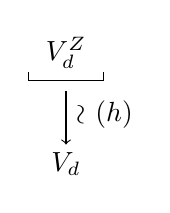
\begin{tikzpicture}[baseline=(top.base),x=1cm,y=1cm]
  \node (top) at (0,0) {$V_d^Z$};
  \draw (-.48,-.25)--(-.48,-.36)--(.48,-.36)--(.48,-.25);
  \draw[->] (0,-.49)--(0,-1.17);
  \node[rotate=90] at (.21,-.79) {$\sim$};
  \node at (.61,-.79) {$(h)$};
  \node at (0,-1.42) {$V_d$};
\end{tikzpicture}
\]
\margin{si $J\prec L$, $J$ et $L$ des bandes et si $Z$ contient $\deleted{X_J^*\unsure{\cap}}X_L^*$, donc contient $X_{i_n}^*$ si $d=(i_0,\mathord{\cdot}\mathord{-},i_n)$}

\deleted{clairement} \inserted{donc si} \inserted{$J,L$ des bandes et $J\prec L$, et si} $Z$ contient $\deleted{X_J^*\unsure{\cap}}X_L^*$, on aura
\[
(110)\qquad V_{J,L}^Z\overset{(\overset h\sim)}{\hookrightarrow}V_{\unsure{J|\square},L}
\]
en particulier
\[
(111)\qquad V_{J\unsure{,|0}}^L\left(\overset{\mathrm{déf}}=V_{J,L}^{X_L^*}\right)\overset{(\overset h\sim)}{\hookrightarrow}V_{J,L}
\]

Soient
\[
(112)\qquad J_0\prec J_1\prec \mathord{\cdot}\mathord{-}\prec J_n
\]
des bandes, on posera
\[
(113)\qquad\begin{aligned}
V_{J_0,\mathord{\cdot}\mathord{-},J_n}&=V_{J_0}\cap \mathord{-}\mathord{-}\cap V_{J_n}\\
&=\bigcup_{\substack{j_0\in J_0\\\mathord{\cdot}\mathord{\cdot}\mathord{-}\\j_n\in J_n}}V_{j_0j_1\mathord{\cdot}\mathord{-}j_n}\\
&=\underset{\substack{d\in\mathrm{Drap}(J_0\cup J_1\cup \mathord{\cdot}\mathord{-}\cup J_n)\\d\cap J_0\ne\phi,\mathord{\cdot}\mathord{\cdot}\mathord{-},d\cap J_n\ne\phi}}{\lim_{\longrightarrow}}V_d
\end{aligned}
\]

% The following three-line block is entirely canceled. The lower stars are placed below the baseline; their attachment remains uncertain.
\[
\begin{aligned}
\deleted{X}&\deleted{=\unsure{\overline{V}_{J}^{L}}}\\
&\deleted{\unsure{Z\cap V_J}}\\
&\deleted{=\unsure{{}_{*}X\cup V_{J\cup L}\cap{}_{*}V_L}}
\end{aligned}
\]
\margin{98}

\cotefile{151}

\scanpage{3}

\diagram{\begin{tikzcd}[ampersand replacement=\&,column sep=large,row sep=small]
E_0\arrow[r,bend left=50,"\delta_0"]\&E_1\arrow[l,shift right=1.2ex,"p_0"']\arrow[l,shift left=1.2ex,"p_1"]\arrow[r,bend left=50,"{\delta_1,\delta_2,\delta_3}"]\arrow[r,bend left=60]\arrow[r,bend left=70]\&E_2\arrow[l,shift right=2.2ex,"p_{12}"']\arrow[l,"p_{23}"']\arrow[l,shift left=2.2ex,"p_{13}"]\\
\&\mathcal G_2\arrow[d,phantom,"\in" rotate=90]\&\mathcal G_3\arrow[d,phantom,"\in" rotate=90]\\
\&\sigma\&\overbrace{\rho,\sigma_1,\sigma_2,\sigma_3}\\
\&\&\rho^2
\end{tikzcd}}
\deleted{\diagram{\begin{tikzcd}[ampersand replacement=\&,column sep=large]
{}\arrow[r,bend right=40,"\unsure{\delta_1}"']\arrow[r,bend right=55,"\unsure{\delta_2}"']\arrow[r,bend right=70,"\delta_3"']\&{}
\end{tikzcd}}}
\[\boxed{\begin{aligned}
\delta_3(x,y)&=(x,x,y)\\
\delta_1(x,y)&=(y,x,x)\\
\delta_2(x,y)&=(x,y,x)
\end{aligned}}\]
\margin{\deleted{$\delta_1\sigma(x,y)=(y,y,x)$}\quad $=$\\$\unsure{\sigma|\delta}_3\delta_3$}
\mspage{\textcircled{1}}
\[p_{\unsure{1|0}}=p_0\sigma,\quad p_0=p_1\sigma\]
\[\boxed{\begin{aligned}
p_{12}(x,y,z)&=(x,y)\\
p_{\deleted{\unsure{21}}\inserted{23}}(x,y,z)&=(y,z)\\
p_{31}(x,y,z)&=(z,x)
\end{aligned}}\]
\margin{$\rho(x,y,z)=(y,z,x)$}
\deleted{\[p_{12}=p_{23}\]}
\[\boxed{\left\{\begin{aligned}
p_{23}&=p_{12}\rho\\
p_{31}&=p_{23}\rho=p_{12}\rho^2\\
p_{12}&=p_{31}\rho=p_{23}\rho^2
\end{aligned}\right.}\]
\[\begin{aligned}
\sigma p_{12}&=p_{12}\sigma_3\\
\sigma p_{23}&=p_{23}\sigma_1\\
\sigma p_{31}&=p_{31}\sigma_2
\end{aligned}\]
\deleted{\[(x,y,z)\longrightarrow(y,z,x)\longrightarrow(y,z)\]}
\[\left\{\begin{aligned}
\delta_1&=\rho\delta_2=\rho^2\delta_3\\
\delta_2&=\rho\delta_3=\rho^2\delta_1\\
\delta_3&=\rho\delta_1=\rho^2\delta_2{}^{\unsure{a}}
\end{aligned}\right.\]

\deleted{\unsure{a}} Il suffit de avoir $p_0,p_{12},\delta_0,\delta_1$ entre les trois ensembles $E_0$, $(E_1,\mathcal G_2)$, $(E_2,\mathcal G_3)$, avec les relations
\[\boxed{p_0\delta_0=\mathrm{id}_{E_0}}\quad\deleted{\unsure{p_1\delta_0|p_{12}\delta_0}}\]
\[\delta_0p_0=p_{12}\underbrace{\delta_3}_{\rho^{\deleted{\unsure{2|\sigma}}}\delta_1}=\underbrace{p_{23}}_{p_{12}\rho}\underbrace{\delta_1}_{\deleted{\unsure{\rho}}}=\underbrace{p_{31}}_{p_{12}\rho^2}\underbrace{\delta_2}_{\rho^2\delta_1}\]
\[\boxed{\sigma\delta_0=\delta_0}\]
\deleted{\[\text{i.e.}\quad\underbrace{\delta_0p_0}=\underbrace{p_{12}\delta_1}_{\sigma}=\underbrace{p_{12}\rho\delta_1}_{\mathrm{id}}=\underbrace{p_{12}\rho^2\delta_1}\]}
\deleted{\[\underbrace{(p_{12}\rho)}_{p_{23}}\delta_1\overset{??}{\ne}\unsure{p_{22}|p_{12}|p_{23}}(\underbrace{\rho\delta_1}_{\delta_2})\]}
\[\boxed{\begin{aligned}
\delta_0p_0&=p_{12}\overbrace{\rho\delta_1}^{\delta_3}\\
\mathrm{id}_{E_1}&=p_{12}\underbrace{\rho_{\deleted{\unsure{1}}}^{2}\delta_1}_{\delta_2}\\
\sigma&=p_{12}\delta_1
\end{aligned}}\]
\margin{$\boxed{\sigma_3\delta_1=\delta_1}$\\$\boxed{p_{12}\sigma_3=\sigma p_{12}}$}
\deleted{$\unsure{(\mathrm{Ens})|\mathrm{ens}}$}
\diagram{\begin{tikzcd}[ampersand replacement=\&,column sep=large,row sep=small,execute at end picture={\draw (current bounding box.south west) rectangle (current bounding box.north east);}]
\deleted{\unsure{\mathcal G|\mathfrak S}_{\unsure{2|1}}}\&\mathcal G_2\&\mathcal G_3\\
E_0\arrow[r,bend right=30,"\delta_0"']\&E_1\arrow[l,"p_0"']\arrow[r,bend right=30,"\delta_1"']\&E_2\arrow[l,"p_{12}"']
\end{tikzcd}}
\[\boxed{\rho\delta_1\delta_0=\sigma_1\delta_1\delta_0=\delta_1\delta_0}\]
\[\underbrace{p_0p_{12}}_{p_{\unsure{2|1}}}=p_0\overbrace{\underbrace{p_{12}\deleted{\unsure{\sigma}}\rho^2}_{p_{31}}\sigma_2}^{p_{12}}\]
\margin{2}

\scanpage{4}
% The letter is upside down in the source scan. Its typed reading order is restored here.
\hrule
\begin{tabular}{p{.47\linewidth}p{.47\linewidth}}
\textbf{ACADEMIE D'AIX-MARSEILLE} & AVIGNON le 6 décembre 1990\\
\rule{3cm}{.4pt}&\\
\textbf{INSPECTION ACADEMIQUE} & Jacques ROUX, responsable\\
\textbf{DE VAUCLUSE}&départemental de l'Action\\
\rule{1cm}{.4pt}&Culturelle,\\[1em]
C.D.A.C.N°16&à\\[1em]
&M
\end{tabular}

\uline{OBJET} : Projets d'Action Educative Collège.\\
Année scolaire 1990/1991

L'attribution des aides aux P.A.E. se déroulera cette année en deux temps :

\begin{tabular}{l p{.72\linewidth}}
DECEMBRE & - instruction des dossiers\\
&par l'Inspection Académique\\[1em]
&propositions à la M.I.A.D.A.C.\\[1em]
JANVIER & - Monsieur le Recteur attribue\\
&une aide globalisée à Monsieur\\
&l'Inspecteur d'Académie.
\end{tabular}

Une commission se réunit vers le 15 janvier 1991, afin d'assurer la ventilation des aides au niveau du département. Je vous demanderai alors de participer à cette Commission.

P/L'Inspecteur d'Académie

% Unreadable autograph with a long looped flourish; it is not a cancellation of the typed text.
\handwritten{\illegible{1}}

% A separate lower line is clipped to a few stroke tops at the scan edge. No complete word is reconstructed.
\illegible{1}
\margin{3}

\scanpage{5}

\[\deleted{\begin{array}{ccc}
p_0/p_1&p_{12}\quad p_{23}\quad p_{31}&\delta_1\quad\delta_2\quad\delta_3\\
\delta_0&\deleted{\unsure{\sigma p_{12}\quad\sigma p}}&\\
&p_{21}\quad p_{32}\quad p_{13}&
\end{array}}\]
\mspage{\textcircled{2}}
\[\deleted{\delta_0p_0},\deleted{\delta_0p_1},\quad\mathrm{id},\sigma\]
\diagram{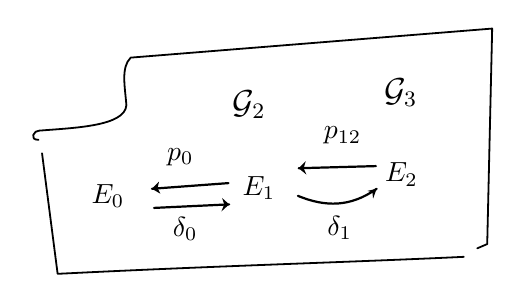
\begin{tikzpicture}[x=.009cm,y=-.009cm,line cap=round,line join=round]
\node at (113,251) {$E_0$};
\node at (326,240) {$E_1$};
\node at (527,221) {$E_2$};
\node at (312,123) {\large$\mathcal G_2$};
\node at (526,105) {\large$\mathcal G_3$};
\draw[line width=.8pt] (283,233) -- (175,241);
\fill (175,241) -- (185,231) -- (183,240) -- (187,248) -- cycle;
\node at (215,196) {$p_0$};
\draw[line width=.8pt] (178,268) -- (284,263);
\fill (284,263) -- (274,254) -- (277,263) -- (273,273) -- cycle;
\node at (222,297) {$\delta_0$};
\draw[line width=.8pt] (491,209) -- (382,212);
\fill (382,212) -- (392,202) -- (389,212) -- (393,221) -- cycle;
\node at (444,166) {$p_{12}$};
\draw[line width=.8pt] (381,251) .. controls (420,267) and (455,267) .. (492,241);
\fill (492,241) -- (479,244) -- (486,246) -- (487,255) -- cycle;
\node at (440,296) {$\delta_1$};
\draw[line width=.65pt] (15,172) .. controls (1,172) and (9,158) .. (16,159)
 .. controls (65,155) and (137,153) .. (139,123)
 .. controls (137,97) and (131,70) .. (145,56)
 -- (655,15) -- (648,319) -- (634,325);
\draw[line width=.65pt] (20,191) -- (42,361)
 .. controls (260,350) and (470,344) .. (615,337);
\end{tikzpicture}}
\[\deleted{\delta_1p_{12}}\]
\[\boxed{\begin{aligned}p_0\delta_0&=\mathrm{id}_{E_0}\\\sigma\delta_0&=\delta_0\end{aligned}}\]
\[\boxed{\begin{aligned}
p_{12}\delta_1&=\sigma\qquad\text{(involution}\\
p_{12}\overset{\deleted{\unsure{\mathrm{id}}}}{\underbrace{\rho\delta_1}_{\delta_3}}&=\delta_0p_0\qquad\text{(idempotent)}\\
p_{12}(\underbrace{\rho^2\delta_1}_{\delta_2})&=\mathrm{id}
\end{aligned}}\]
\margin{$\boxed{\deleted{p_0/p_1}}$\\\diagram{\begin{tikzcd}[execute at end picture={\foreach \ovalnode in {ovalp}{\begingroup\pgfextractx{\dimen0}{\pgfpointdiff{\pgfpointanchor{\ovalnode}{west}}{\pgfpointanchor{\ovalnode}{east}}}\pgfextracty{\dimen2}{\pgfpointdiff{\pgfpointanchor{\ovalnode}{south}}{\pgfpointanchor{\ovalnode}{north}}}\dimen0=.7071067812\dimen0\dimen2=.7071067812\dimen2\draw (\ovalnode.center) ellipse[x radius=\the\dimen0,y radius=\the\dimen2];\endgroup}}]|[alias=ovalp,rectangle,draw=none]|p_0,p_1\end{tikzcd}}}
\diagram{\begin{tikzcd}[ampersand replacement=\&,column sep=large,row sep=small,execute at end picture={\foreach \ovalnode in {ovald,ovaldp,ovalpp}{\begingroup\pgfextractx{\dimen0}{\pgfpointdiff{\pgfpointanchor{\ovalnode}{west}}{\pgfpointanchor{\ovalnode}{east}}}\pgfextracty{\dimen2}{\pgfpointdiff{\pgfpointanchor{\ovalnode}{south}}{\pgfpointanchor{\ovalnode}{north}}}\dimen0=.7071067812\dimen0\dimen2=.7071067812\dimen2\draw (\ovalnode.center) ellipse[x radius=\the\dimen0,y radius=\the\dimen2];\endgroup}}]
\boxed{\begin{gathered}\sigma_1\delta_1=\delta_1\\p_{12}\sigma_3=\underbrace{\sigma p_{12}}_{p_{21}}\end{gathered}}\&|[alias=ovald,rectangle,draw=none]|\delta_1,\delta_2,\delta_3\arrow[l,bend right=15,shorten <=1em]\&|[alias=ovaldp,rectangle,draw=none]|\begin{gathered}\delta'_1=\delta_1\sigma\\\delta'_2=\delta_2\sigma\\\delta'_3=\delta_3\sigma\end{gathered}\\
\&|[alias=ovalpp,rectangle,draw=none]|\begin{gathered}p_{12},p_{23},p_{31},\unsure{{}^3}\\p_{21},p_{32},p_{13}\end{gathered}\&
\end{tikzcd}}
\[\boxed{\begin{gathered}
\rho(\delta_1\delta_0)=\sigma_1(\delta_1\delta_0)=\delta_1\delta_0\\
\text{i.e.}\qquad g(\delta_1\delta_0)=\delta_1\delta_0\quad\text{pour }g\in\mathcal G_3
\end{gathered}}\]
\[\boxed{p_0p_{12}\sigma_1=\underbrace{p_0p_{12}}_{\unsure{q_1|p_1}}}\]
\margin{\diagram{\begin{tikzcd}[execute at end picture={\foreach \ovalnode in {ovalq}{\begingroup\pgfextractx{\dimen0}{\pgfpointdiff{\pgfpointanchor{\ovalnode}{west}}{\pgfpointanchor{\ovalnode}{east}}}\pgfextracty{\dimen2}{\pgfpointdiff{\pgfpointanchor{\ovalnode}{south}}{\pgfpointanchor{\ovalnode}{north}}}\dimen0=.7071067812\dimen0\dimen2=.7071067812\dimen2\draw (\ovalnode.center) ellipse[x radius=\the\dimen0,y radius=\the\dimen2];\endgroup}}]|[alias=ovalq,rectangle,draw=none]|q_1,q_2,q_3\end{tikzcd}}}
\margin{4}

\scanpage{6}
% The source letter is upside down; typed reading order is restored.

\hrule
\begin{tabular}{p{.47\linewidth}p{.47\linewidth}}
\textbf{ACADEMIE D'AIX-MARSEILLE} & AVIGNON le 6 décembre 1990\\
\rule{3cm}{.4pt}&\\
\textbf{INSPECTION ACADEMIQUE} & Jacques ROUX, responsable\\
\textbf{DE VAUCLUSE}&départemental de l'Action\\
\rule{1cm}{.4pt}&Culturelle,\\[1em]
C.D.A.C.N°16&à\\[1em]
&M
\end{tabular}

\uline{OBJET} : Projets d'Action Educative Collège.\\
Année scolaire 1990/1991

L'attribution des aides aux P.A.E. se déroulera cette année en deux temps :

\begin{tabular}{l p{.72\linewidth}}
DECEMBRE & - instruction des dossiers\\
&par l'Inspection Académique\\[1em]
&propositions à la M.I.A.D.A.C.\\[1em]
JANVIER & - Monsieur le Recteur attribue\\
&une aide globalisée à Monsieur\\
&l'Inspecteur d'Académie.
\end{tabular}

Une commission se réunit vers le 15 janvier 1991, afin d'assurer la ventilation des aides au niveau du département. Je vous demanderai alors de participer à cette Commission.

P/L'Inspecteur d'Académie

% Unreadable autograph; its looped flourish is not a cancellation.
\handwritten{\illegible{1}}

% A separate line below the autograph is clipped to character tops. No missing lower letter parts are reconstructed.
\illegible{1}
\margin{5}

\scanpage{7}
\mspage{\textcircled{3}}

% The upper calculations are canceled en bloc by three long oblique strokes
% and a sweeping left/bottom boundary. Each complete diagram, including its
% arrow paths, is wrapped in deleted; mbox keeps its drawing indivisible.
\[
\deleted{p_0p_{12}=p_0p_{13}=p_0\underbrace{p_{12}\rho^2}_{p_{31}}\sigma_2}
\qquad
\deleted{\rho^2\sigma_2=\sigma_3\rho^2}
\]
\diagram{\deleted{\mbox{\begin{tikzcd}[ampersand replacement=\&,row sep=small,column sep=large]
(x,y,z)\arrow[r,mapsto]\&(z,y,x)\&{}\\
{}\arrow[r]\&(x,z)\arrow[r]\&x
\end{tikzcd}}}}
\[\deleted{p_0p_{12}\sigma_1=p_0p_{12}}\]
\[\deleted{(x,x,y)}\]
% The continuation shaft has a separate tail bar and a small loop at its
% right endpoint. It is not replaced by the clear chevron of the row above.
\diagram{\deleted{\mbox{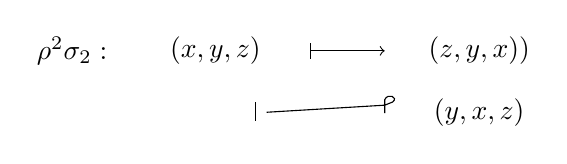
\begin{tikzpicture}[x=1cm,y=1cm]
\node[anchor=east] at (-0.8,0) {$\rho^2\sigma_2:$};
\node at (0.45,0) {$(x,y,z)$};
\node at (3.8,0) {$(z,y,x))$};
\draw[|->] (1.65,0)--(2.6,0);
\draw (0.96,-0.89)--(0.96,-0.65);
\draw (1.1,-0.78)--(2.6,-0.69);
\draw (2.6,-0.79)--(2.6,-0.62)
  .. controls (2.64,-0.53) and (2.78,-0.59) .. (2.7,-0.65)
  --(2.6,-0.69);
\node at (3.8,-0.78) {$(\uline{y,x},z)$};
\end{tikzpicture}}}}
\[
\begin{array}{ll}
\deleted{\delta_1\sigma=(x,y,y)}&{}\\[0.7ex]
\deleted{(x,\unsure{x},y)}&\qquad\deleted{z,x,y}\\[0.7ex]
\deleted{(y,y,x)}&{}
\end{array}
\]
% Tail bar and square downturned terminal are both visible; no chevron
% is supplied to the last coordinate mapping.
\diagram{\deleted{\mbox{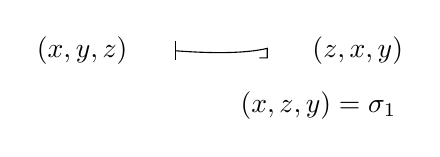
\begin{tikzpicture}[x=1cm,y=1cm]
\node at (0,0) {$(x,y,z)$};
\node at (3.5,0) {$(z,x,y)$};
\draw (1.18,-0.12)--(1.18,0.12);
\draw (1.18,0) .. controls (1.7,-0.04) and (2.1,-0.03) .. (2.35,0.03)
  --(2.35,-0.09)--(2.25,-0.09);
\node at (3.0,-0.7) {$(x,z,y)=\sigma_1$};
\end{tikzpicture}}}}

\mspage{\textcircled{3}}
Si $E_0$ est réduit à un p\textsuperscript{t}, donc par $\delta_0,\delta_1\delta_0$ $E_1,E_2$ deviennent des ens. pointés, et $\mathcal G_2,\mathcal G_3$ respectent la ponctuation.
\margin{(``ponctués'')}
\deleted{\unsure{Donc.|On a.}}
$\deleted{\delta_1}$ \deleted{respecte \unsure{les|le}}
Donc, en plus des opérations de $\mathcal G_2,\mathcal G_3$, on a
\diagram{\begin{tikzcd}[ampersand replacement=\&,column sep=large]
E_1\arrow[r,bend right=35,"\delta_1"']\&E_2\arrow[l,"p_{12}"']
\end{tikzcd}}
, où $\delta_1$ \inserted{et $p_{12}$} respect\unsure{ent}%
% The terminal low loop, high arch and return touch the right paper edge;
% the compressed n/t cannot be separated securely. No punctuation supplied.
\ les ponctuations, et où $p_{12},\delta_1$ satisfont aux cinq relations supplémentaires
\[\boxed{\begin{aligned}
p_{12}\delta_1&=\sigma\\
p_{12}\underbrace{\rho\delta_1}_{\delta_3}&=\text{application constante de valeur }e_1\quad\text{(p\textsuperscript{t} marqué de }E_1\text{)}\\
p_{12}\underbrace{\rho^2\delta_1}_{\delta_2}&=\mathrm{id}_{E_1}\\
\sigma_1\delta_1&=\delta_1\\
p_{12}\sigma_3&=\sigma p_{12}
\end{aligned}}\]
% This smaller compartment sits inside the lower right of the outer box,
% sharing its right and bottom boundary; the following marginal items are
% adjacent to its three rows. Their textual state is preserved separately.
\margin{$\boxed{\begin{aligned}
p_{12}\delta_2&=\mathrm{id}_{E_1}\\
p_{12}\underbrace{\rho\delta_2}_{\delta_1}&=\sigma\\
p_{12}\underbrace{\rho^2\delta_2}_{\delta_3}&=e_1\quad\text{(application de }E_1\text{ sur }e_1\text{)}
\end{aligned}}$}
\margin{$\uline{p_{12}\sigma_3=\sigma p_{11}}$\\
$\sigma_2\delta_2=\delta_2$\\
$\deleted{p_{12}\sigma_3\unsure{=\sigma}p_{12}}$\\
$\deleted{\unsure{\mathrm{id}}}$\\
\begin{tikzcd}[ampersand replacement=\&,column sep=large]
E_1\arrow[r,bend right=12,"\delta_1"']\&E_2\arrow[l,"p_{12}"']
\end{tikzcd}}
\margin{6}
